%==============================================================================
%vvvvvvvvvvvvvvvvvvvvvvvvvvvvvvvvvvvvvvvvvvvvvvvvvvvvvvvvvvvvvvvvvvvvvvvvvvvvvv

\documentclass{beamer}
\usepackage[utf8]{inputenc}
\usepackage[ngerman]{babel} % neue deutsche Rechtschreibung 
\usepackage{babelbib}       % deutsches Literaturverzeichnis
\usepackage{verbatim} 


% Background
\usepackage{tikz}
\usetikzlibrary{shapes.geometric, arrows}
\usetikzlibrary{fadings}
\setbeamertemplate{background}{
\begin{tikzpicture}
\path (0,0) rectangle (\paperwidth,\paperheight);
\node[scope fading=west,inner sep=0pt,outer sep=0pt,anchor=north east] at(\paperwidth*1.3,\paperheight*0.83) {
\includegraphics[height=\paperheight]{pics/uni}};
\end{tikzpicture}
}

\PassOptionsToPackage{usenames}{color} 
\usepackage{color} 
\usepackage[usenames]{color} 


%^^^^^^^^^^^^^^^^^^^^^^^^^^^^^^^^^^^^^^^^^^^^^^^^^^^^^^^^^^^^^^^^^^^^^^^^^^^^^^
%==============================================================================
%vvvvvvvvvvvvvvvvvvvvvvvvvvvvvvvvvvvvvvvvvvvvvvvvvvvvvvvvvvvvvvvvvvvvvvvvvvvvvv

\usetheme{default}
\usecolortheme{seagull}

% Remove navigation
\beamertemplatenavigationsymbolsempty
% \setcounter{tocdepth}{2}
\usecaptiontemplate{
  \tiny
  \insertcaption
}
\setbeamertemplate{footline}[frame number] 

% Use bullet as item for lists
\setbeamertemplate{itemize items}{$\bullet$}

% %\setbeamertemplate{itemize subitem}{{\tiny $\spadesuit$}}
% %\setbeamertemplate{itemize subsubitem}{{\tiny $\heartsuit$}}
% \setbeamertemplate{footline}[frame number]
% \setbeamertemplate{sections/subsections in toc}[circle]{}

%^^^^^^^^^^^^^^^^^^^^^^^^^^^^^^^^^^^^^^^^^^^^^^^^^^^^^^^^^^^^^^^^^^^^^^^^^^^^^^
%==============================================================================




\title{Per-Circuit TCP-over-IPsec Transport\\for Anonymous Communication Overlay Networks}   
\author{Manuel Schneider}
\institute{Albert Ludwigs Universität - Institut für Informatik} 
\date{\today} 

%==============================================================================
%//////////////////////////////////////////////////////////////////////////////
%//////////////////////////////////////////////////////////////////////////////
%//////////////////////////////////////////////////////////////////////////////
\begin{document}%//////////////////////////////////////////////////////////////
%//////////////////////////////////////////////////////////////////////////////
%//////////////////////////////////////////////////////////////////////////////
%//////////////////////////////////////////////////////////////////////////////
%==============================================================================

%30 sek
\begin{frame}[plain]
  \titlepage
\end{frame}


% \begin{frame}[plain]{Motivation}
%   \begin{figure}
%     \includegraphics[width=0.4\textwidth]{pics/phonelatency}
%   \end{figure}
%   \begin{itemize}
%     \item Tor Latency 1s $\pm$ 0.5s
%     \item bla
%   \end{itemize}
% \end{frame}

%==============================================================================
%//////////////////////////////////////////////////////////////////////////////
\section{TOR}
%//////////////////////////////////////////////////////////////////////////////
%==============================================================================

\begin{frame}{\textsc{Tor} - Architektur/Terminologie}
  \begin{figure}
    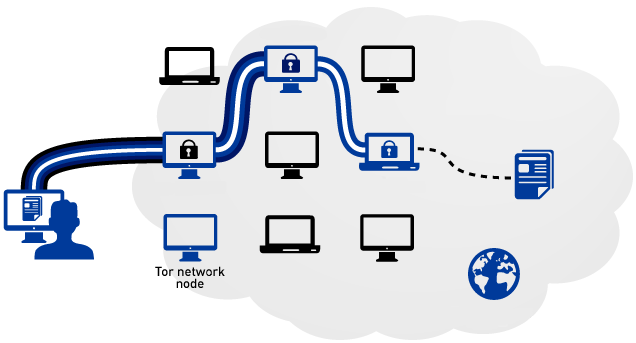
\includegraphics[width=0.9\textwidth]{pics/tor}
  \end{figure}
\end{frame}


% \begin{frame}{Cells - Das \textsc{Tor} Tranportmittel}{\secname}
%     \begin{figure}
%       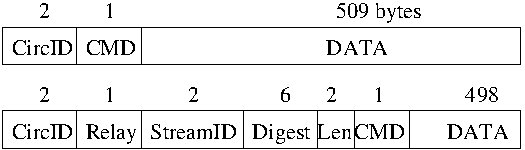
\includegraphics[width=0.6\textwidth]{pics/cell}
%       \hspace{0.1cm}
%       {\tiny Quelle: \cite{tor}}
%     \end{figure}
%     \begin{block}{Control Cell}
%       \begin{itemize}
%         \item Dienen dem Management der Circuits
%         \begin{itemize}
%           \item Aufbau, Abbau, Keepalive
%         \end{itemize}
%         \item Werden vom Onion Router interpretiert, der sie empfängt
%       \end{itemize}
%     \end{block} 
%     \begin{block}{Relay Cell}
%       \begin{itemize}
%         \item Zur Weiterleitung der Daten auf dem Circuit
%         \item Zusätzlicher Relay Header
%       \end{itemize}
%     \end{block}
% \end{frame}


\begin{frame}{Circuits}{\secname}
  \begin{figure}
    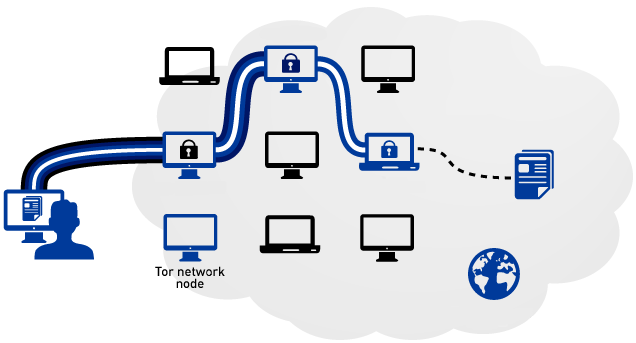
\includegraphics[width=.7\textwidth]{pics/tor}
  \end{figure}
  \begin{itemize}
    \item Werden Hop-by-hop aufgebaut
    \begin{itemize}
      \item Mit jedem Knoten wird ein Schlüssel ausgehandelt
    \end{itemize}
    \item Üblicherweise drei: Entry\-, Middle-, Exit Node
    \item Werden nach einem Zeitintervall oder Fehler gewechselt
    \item Werden auf Vorrat angelegt (Performance)
  \end{itemize}
\end{frame}

% \begin{frame}{Cell Relaying / Onion Routing}{\secname}
% Hier noch tolles bild mit circid
% 
%   $$CircID | Relay | {\color{red}\{}{\color{green}\{}{\color{blue}\{}Relayheader| DATA{\color{blue}\}_{K_3}}{\color{green}\}_{K_2}}{\color{red}\}_{K_1}}$$
%   $$CircID | Relay | {\color{green}\{}{\color{blue}\{}Relayheader| DATA{\color{blue}\}_{K_3}}{\color{green}\}_{K_2}}$$
%   $$CircID | Relay | {\color{blue}\{}Relayheader| DATA{\color{blue}\}_{K_3}}$$
%   $$CircID | Relay | Relayheader| DATA$$
% \end{frame}

\begin{frame}{Circuit construction}{\secname}
  \begin{center}
    \begin{tikzpicture}%[font=\tiny]
      \draw[draw,line width=1.2pt] (0,0) -- (0,1) node[above] {OP};
      \draw[draw,line width=1.2pt] (3,0) -- (3,1) node[above] {OR$_1$};
      \draw[draw,line width=1.2pt] (6,0) -- (6,1) node[above] {OR$_2$};
      \draw[draw,line width=1.2pt] (9,0) -- (9,1) node[above] {OR$_3$};
      \draw[-latex] (0,0.75) -- node[anchor=south, font=\tiny]{Create} (3,0.75);
      \draw[latex-] (0,0.25) -- node[anchor=south, font=\tiny]{Created} (3,0.25);
    \end{tikzpicture}
  \end{center}

  \begin{block}{Circuit Erweiterung}
    \begin{itemize}
      \item OP sendet \textcolor{brown}{Create Control} Cell an OR$_1$
      \item OR$_1$ bestätigt mit \textcolor{brown}{Created Control} Cell
      \item Wenn schon eine Verbindung besteht wird diese genutzt
      \item Schlüsselaustausch: OP und OR$_1$ teilen Schlüssel K$_1$
      \item Beide merken sich Circuit Identifier
    \end{itemize}
  \end{block}
\end{frame}



\begin{frame}{Circuit construction}{\secname}
  \only<1>
  {
  \begin{center}
    \begin{tikzpicture}%[font=\tiny]
      \draw[draw,line width=1.1pt] (0,0) -- (0,1) node[above] {OP};
      \draw[draw,line width=1.1pt] (3,0) -- (3,1) node[above] {OR$_1$};
      \draw[draw,line width=1.1pt] (6,0) -- (6,1) node[above] {OR$_2$};
      \draw[draw,line width=1.1pt] (9,0) -- (9,1) node[above] {OR$_3$};
      \draw[dotted,-latex] (0,0.9) -- node[anchor=south, font=\tiny]{Relay {\color{blue}\{Extend\}$_{K_1}$}}   (3,0.9);
      \draw[dotted,latex-] (0,0.1) -- node[anchor=south, font=\tiny]{Relay {\color{blue}\{Extended\}$_{K_1}$}} (3,0.1);
      \draw[-latex] (3,0.8) -- node[anchor=south, font=\tiny]{Create} (6,0.8);
      \draw[latex-] (3,0.2) -- node[anchor=south, font=\tiny]{Created} (6,0.2);
    \end{tikzpicture}
  \end{center}
  }
  \only<2>
  {
  \begin{center}
    \begin{tikzpicture}%[font=\tiny]
      \draw[draw,line width=1.2pt] (0,0) -- (0,1) node[above] {OP};
      \draw[draw,line width=1.2pt] (3,0) -- (3,1) node[above] {OR$_1$};
      \draw[draw,line width=1.2pt] (6,0) -- (6,1) node[above] {OR$_2$};
      \draw[draw,line width=1.2pt] (9,0) -- (9,1) node[above] {OR$_3$};
      \draw[dotted,-latex] (0,0.9) -- node[anchor=south, font=\tiny]{Relay {\color{red}\{\{Extend\}$_{K_2}$\}$_{K_1}$}}   (3,0.9);
      \draw[dotted,latex-] (0,0.1) -- node[anchor=south, font=\tiny]{Relay {\color{red}\{\{Extended\}$_{K_2}$\}$_{K_1}$}} (3,0.1);
      \draw[dotted,-latex] (3,0.8) -- node[anchor=south, font=\tiny]{Relay {\color{blue}\{Extend\}$_{K_2}$}}   (6,0.8);
      \draw[dotted,latex-] (3,0.2) -- node[anchor=south, font=\tiny]{Relay {\color{blue}\{Extended\}$_{K_2}$}} (6,0.2);
      \draw[-latex] (6,0.7) -- node[anchor=south, font=\tiny]{Create}   (9,0.7);
      \draw[latex-] (6,0.3) -- node[anchor=south, font=\tiny]{Created} (9,0.3);
    \end{tikzpicture}
  \end{center}
  }
  \begin{block}{Relay Erweiterung}
    \begin{itemize}
      \item OP sendet \textcolor{brown}{Extend Relay} Cell an OR$_1$
      \item OR$_1$ erweitert den Circuit zu OR$_2$ (\textcolor{brown}{Create})
      \item OR$_1$ leitet die Antwort in einer\\ \textcolor{brown}{Extended Relay} Cell an OP zurück  
      \item OP und OR$_2$ teilen einen gemeinsamen Schlüssel K$_2$
    \end{itemize}
  \end{block}
\end{frame}


\begin{frame}{Cross Circuit Interference Problem}{\secname}
  \begin{figure}
    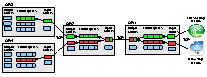
\includegraphics[width=0.8\textwidth]{pics/BufferPic.pdf}
    \rotatebox[origin=r]{270}{\tiny Quelle: \cite{pctcp}}
  \end{figure}
  \begin{itemize}
    \item Tritt auf wenn sich verschiedene Circuits\\ eine TCP Verbindung teilen 
    \item Circuits teilen selben Buffer / TCP Mechanismus
    \begin{itemize}
      \item In order delivery
      \item Congestion control
    \end{itemize}
  \end{itemize}
\end{frame}


\begin{frame}{Cross Circuit Interference Problem}{\secname}
  \begin{figure}
    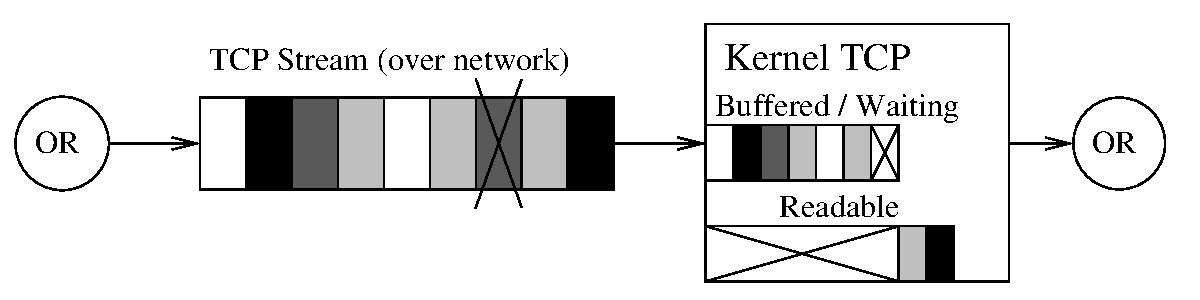
\includegraphics[width=0.7\textwidth]{pics/headonlinevanilla.pdf}
    \rotatebox[origin=r]{270}{\tiny Quelle: \cite{tcp-over-dtls}}
  \end{figure}
  \begin{block}{Head-On-Line Blocking}
    \begin{itemize}
      \item Folge üblicher TCP Arbeitsweise
      \item TCP garantiert eine fehlerfreie und\\Ordnung erhaltende Datenübertragung
      \item Durch eine verlorene Cell werden bereits empfangene\\Nachfolgecells vom Kernel zurückgehalten 
      \begin{itemize}
        \item[$\rightarrow$] Sind diese Cells von einem anderen Circuit,\\äußert sich diese Zeit als Verzögerung
      \end{itemize}
    \end{itemize}
  \end{block}
\end{frame}


%==============================================================================
%//////////////////////////////////////////////////////////////////////////////
\section{PCTCP}
%//////////////////////////////////////////////////////////////////////////////
%==============================================================================


\begin{frame}{Kernel-mode per-circuit TCP}{\secname}
  Problem:
  \begin{itemize}
    \item Gemultiplexte Circuits unterliegen alle\\ den selben TCP Mechanismen
  \end{itemize}
  Lösung in PCTCP:
  \begin{itemize}
    \item Jeder Circuit bekommt eine eigene TCP Verbindung\\(per-circuit TCP)
  \end{itemize}
\end{frame}


\begin{frame}{Recap - Ciruit Construction Vanilla Tor}{\secname}
  \begin{center}
    \begin{tikzpicture}%[font=\tiny]
      \draw[draw,line width=1.2pt] (0,0) -- (0,1) node[above] {OP};
      \draw[draw,line width=1.2pt] (3,0) -- (3,1) node[above] {OR1};
      \draw[draw,line width=1.2pt] (6,0) -- (6,1) node[above] {OR2};
      \draw[draw,line width=1.2pt] (9,0) -- (9,1) node[above] {OR3};
      \draw[-latex] (0,0.75) -- node[anchor=south, font=\tiny]{Create} (3,0.75);
      \draw[latex-] (0,0.25) -- node[anchor=south, font=\tiny]{Created} (3,0.25);
    \end{tikzpicture}
  \end{center}

  \begin{block}{Circuit Erweiterung}
    \begin{itemize}
      \item OP sendet \textcolor{brown}{Create Control} Cell an OR\,1
      \item OR\,1 bestätigt mit \textcolor{brown}{Created Control} Cell
      \item {\color{red}Wenn schon eine Verbindung besteht wird diese genutzt}
      \item Schlüsselaustausch: OP und OR\,1 teilen Schlüssel
      \item Beide merken sich Circuit Identifier
    \end{itemize}
  \end{block}
\end{frame}

\begin{frame}{Recap - Ciruit Construction PCTCP}{\secname}
  \begin{center}
    \begin{tikzpicture}%[font=\tiny]
      \draw[draw,line width=1.2pt] (0,0) -- (0,1) node[above] {OP};
      \draw[draw,line width=1.2pt] (3,0) -- (3,1) node[above] {OR1};
      \draw[draw,line width=1.2pt] (6,0) -- (6,1) node[above] {OR2};
      \draw[draw,line width=1.2pt] (9,0) -- (9,1) node[above] {OR3};
      \draw[-latex] (0,0.75) -- node[anchor=south, font=\tiny]{Create} (3,0.75);
      \draw[latex-] (0,0.25) -- node[anchor=south, font=\tiny]{Created} (3,0.25);
    \end{tikzpicture}
  \end{center}
  \begin{block}{Circuit Erweiterung}
    \begin{itemize}
      \item OP sendet \textcolor{brown}{Create Control} Cell an OR\,1
      \item OR\,1 bestätigt mit \textcolor{brown}{Created Control} Cell
      \item {\color{red}Es wird in jedem Fall eine neue Verbinudung geöffnet}
      \item Schlüsselaustausch: OP und OR\,1 teilen Schlüssel
      \item Beide merken sich Circuit Identifier
    \end{itemize}
  \end{block}
\end{frame}


\begin{frame}{IPSec in PCTCP}{\secname}
  \begin{block}{Warum IPSec?}
    \begin{itemize}
      \item PCTCP: eine TCP Vebindung pro Circuit
      \item TLS verschlüsselt lediglich die Nutzlast/\\ TCP-Header bleibt Klartext
      \begin{itemize}
        \item[$\rightarrow$] Ein Angreifer kann Verbindungen unterscheiden
        \item[$\rightarrow$] Einschränkung der Anonymität
      \end{itemize}
    \end{itemize}
  \end{block} 
\end{frame}


\begin{frame}{Exkurs - IPSec (Internet Protocol Security)}{\secname}
  \begin{itemize}
    \item Arbeitet auf Vermittlungsschicht
    \item Stellt Schutzziele sicher
    \begin{itemize}
      \item Vertraulichkeit
      \item Authentizität
      \item Integrität
    \end{itemize}
    \item Umfasst Protkolle für eine gesicherte Kommunikation
    \begin{itemize}
      \item Authentication Header (AH)
      \item Encapsulating Security Payload (ESP)
    \end{itemize}
    \item Je zwei Betriebsmodi
    \begin{itemize}
      \item Transport Modus
      \item Tunnel Modus
    \end{itemize}
  \end{itemize}
\end{frame}

% 
% \begin{frame}{Exkurs - IPSec  Protokolle}{\secname}
%  \begin{block}{IP Authentication Header (AH)}
%   \begin{itemize}
%    \item Stellt Authentizität und Integrität der Daten sicher
%    \item Authentifiziert Sender 
%    \item Schützt gegen Replay-Angriffe
%    \item Inkompatibel mit Network Adress Translation!
%   \end{itemize}
%  \end{block}
%  \begin{block}{IP Encapsulating Security Payload (ESP)}
%   \begin{itemize}
%    \item Selbes Featureset wie AH
%    \item Stellt zusätzlich Vertraulichkeit der Daten sicher
%   \end{itemize}
%  \end{block}
% \end{frame}
% 
% 
% \begin{frame}{Exkurs - IPSec Betriebsmodi}{\secname}
%   \begin{figure}
%     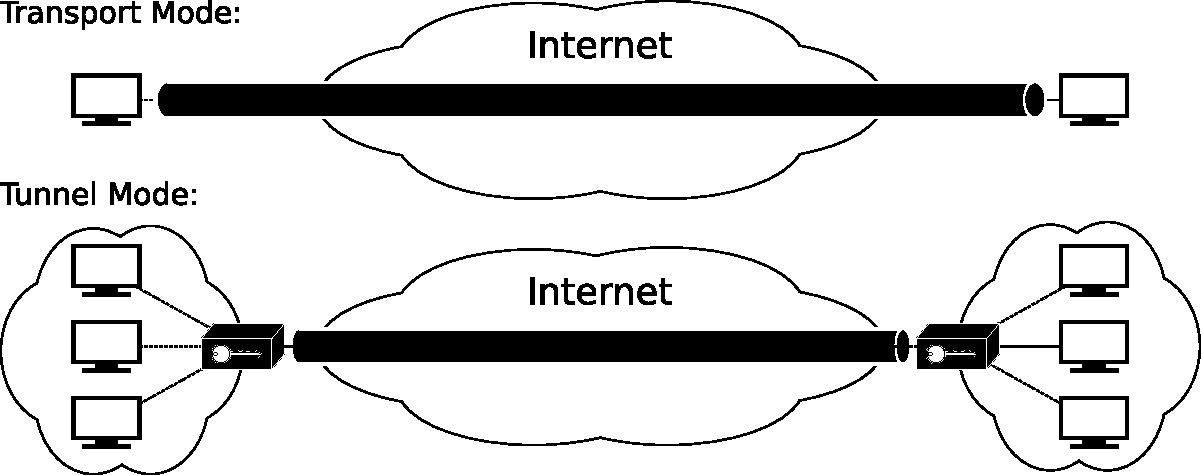
\includegraphics[width=0.7\textwidth]{pics/modes}
%     \caption{Quelle: www.wikimedia.com}
%   \end{figure} 
%   \only<1>
%   {
%     \begin{block}{Transport Modus}
%       \begin{itemize}
% 	\item IP Header bleibt unberührt, auch bei ESP
%       \end{itemize}
%     \end{block} 
%   }
%   \only<2>
%   {
%     \begin{block}{Tunnel Modus}
%       \begin{itemize}
% 	\item Zusätzlicher IP Header 
%       \end{itemize}
%     \end{block} 
%   }
% \end{frame}

\begin{frame}{IPSec in PCTCP}{\secname}
  \begin{figure}[h]
    \begin{center}
      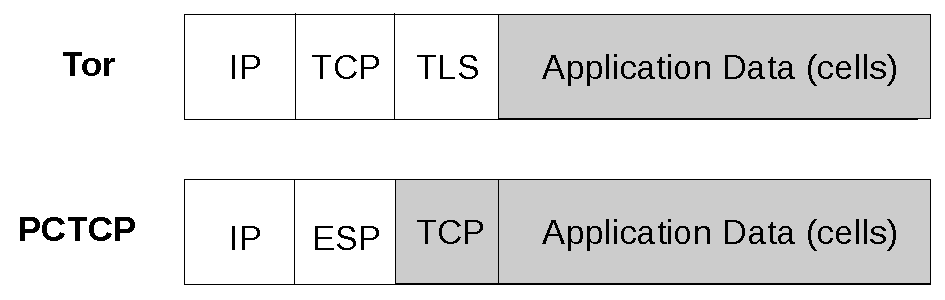
\includegraphics[width=0.7\textwidth]{pics/PCTCP_header.pdf}
      \rotatebox[origin=r]{270}{\tiny Quelle: \cite{pctcp}}
    \end{center}
  \end{figure}
  \begin{itemize}
    \item Encapsulating Security Payload (ESP) im Transport Mode \\
          sorgt für die Vertraulichkeit der Verbindungsdaten
    \item Mit IPSec wird diese Angriffsfläche genommen
    \item TLS ist redundant und wird ausgelassen
  \end{itemize}
\end{frame}


\begin{frame}{PCTCP Überblick}{\secname}
  \begin{figure}
    \begin{center}
      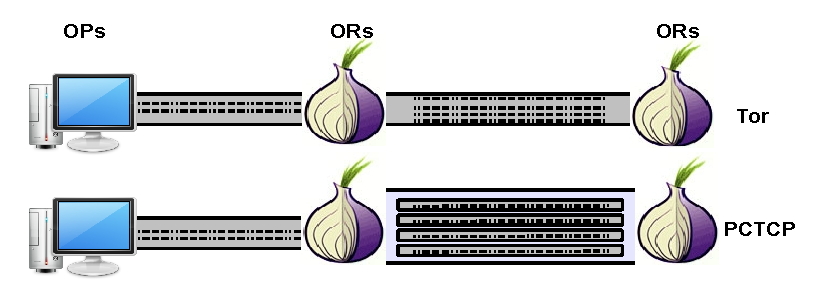
\includegraphics[width=0.9\textwidth]{pics/PCTCP_design.pdf}
      \rotatebox[origin=r]{270}{\tiny Quelle: \cite{pctcp}}
    \end{center}
  \begin{itemize}
    \item ``Kernel-mode per-circuit TCP'' löst das\\
          Cross Circuit Interference Problem
    \item Anstatt TLS sichert IPSec die Schutzziele und sorgt\\
          zusätzlich für die Vertraulichkeit der Verbindungsdaten
  \end{itemize}
  \end{figure} 
\end{frame}


%==============================================================================
%//////////////////////////////////////////////////////////////////////////////
\section{Sicherheit}
%//////////////////////////////////////////////////////////////////////////////
%==============================================================================


\begin{frame}{Socket Exhaustion Attacks}{\secname}
  \begin{itemize}
    \item Sockets sind eine endliche Ressource
    \item Ziel ist den Onion Router außer Kraft zu setzen
    \begin{itemize}
      \item Alle verfügbaren Sockets belegen
      \item So viele Sockets öffen bis das System überlastet wird
    \end{itemize}
    \item Bisher schwierig, wegen Multiplexing der Circuits\\über eine enizige TCP Verbindung
  \end{itemize}
\end{frame}

% \begin{frame}{Socket Exhaustion Attacks}
%   \begin{block}{Angriff auf Exit Nodes}
%     \begin{itemize}
%       \item Jeder Stream öffnet einen Socket an der Exit Node
%       \item Angreifer öffnet Streams über selbe Exit Node,\\ bis diese weitere Streams ablehnt
%       \item Funktioniert auch ohne PCTCP
%       \item Angriff erreicht nicht das komplette Netzwerk
%     \end{itemize}
%   \end{block}
% \end{frame}

\begin{frame}{Socket Exhaustion Attacks}{\secname}
  \begin{figure}[h]
    \begin{center}
      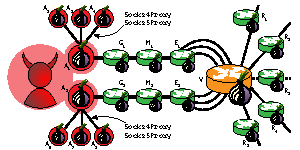
\includegraphics[width=0.7\textwidth]{pics/sniper}
      \rotatebox[origin=r]{270}{\tiny Quelle: \cite{imux}}
    \end{center}
  \end{figure} 
  \begin{block}{Sniper Attack}
    \begin{itemize}
      \item Angriff auf jede Node möglich
      \item Nutzt Tor selbst für den Angriff / Angreifer bleibt anonym
      \item Funktioniert auch ohne PCTCP, aber teuer (1\,OP/Socket)
      \item Mit PCTCP mit einem Onion Proxy möglich
    \end{itemize}
  \end{block}
\end{frame}


\begin{frame}{Socket Exhaustion Attacks}{\secname}
  \begin{block}{PCTCP Socket Exhaustion}
    \begin{itemize}
      \item Basiert auf der Circuit Erweiterung
      \item Circuits werden über Zielknoten aufgebaut
      \item Zielknoten soll Middle Node sein
      \item Angriefer bleibt anonym
      \item Günstig, da nicht mehr ein Onion Proxy\\pro Circuit gebraucht wird
    \end{itemize}
  \end{block}
\end{frame}

% Was konnte man bisher böses anstellen? (Sniper Attack)
% Wie kann man jetzt böses anstellen?
% Warum ist das jetzt auf einmal effizienter?
% Was kann man damit jetzt anfangen?


\begin{frame}{Fazit}
  \begin{itemize}
    \item Einsatz erfordert manuelle Interaktion (IPsec) 
    \begin{itemize}
      \item[$\rightarrow$] Hemmschwelle für Teilnahme steigt
      \item[$\rightarrow$] Gesamtanonymität sinkt
    \end{itemize}
    \item Alternativ: IPSec im Userspace
    \begin{itemize}
      \item Lizenzkompatible Implementierung existiert nicht,\\Eignung vergleichbar mit TCP-over-DLTS
    \end{itemize}
    \item Sicherheitsprobleme sind nicht auf PCTCP bezogen
    \begin{itemize}
      \item Kern des Problems liegt in der\\ ``Ein Circuit Pro TCP''-Verbindung
    \end{itemize}
  \end{itemize}
\end{frame}



%===============================================================================
%///////////////////////////////////////////////////////////////////////////////
%///////////////////////////////////////////////////////////////////////////////
%///////////////////////////////////////////////////////////////////////////////
%===============================================================================

\begin{frame}[plain]{Reference}
  \begin{center}
  Vielen Dank für die Aufmerksamkeit!
  \end{center}
  \tiny
  \bibliographystyle{plain}
  \bibliography{bibliography}
\end{frame}

\nocite{tor}
\nocite{tcp-over-dtls}
\nocite{pctcp}
\nocite{imux}
\nocite{tor_improvements}

%===============================================================================
%///////////////////////////////////////////////////////////////////////////////
%///////////////////////////////////////////////////////////////////////////////
%///////////////////////////////////////////////////////////////////////////////
%///////////////////////////////////////////////////////////////////////////////
\end{document}%/////////////////////////////////////////////////////////////////
%///////////////////////////////////////////////////////////////////////////////
%///////////////////////////////////////////////////////////////////////////////
%///////////////////////////////////////////////////////////////////////////////
%///////////////////////////////////////////////////////////////////////////////
%==============================================/=================================
